\documentclass[border=5pt]{standalone}
\usepackage{tikz}
\usepackage{amsmath}
\usetikzlibrary{patterns, positioning}

\begin{document}

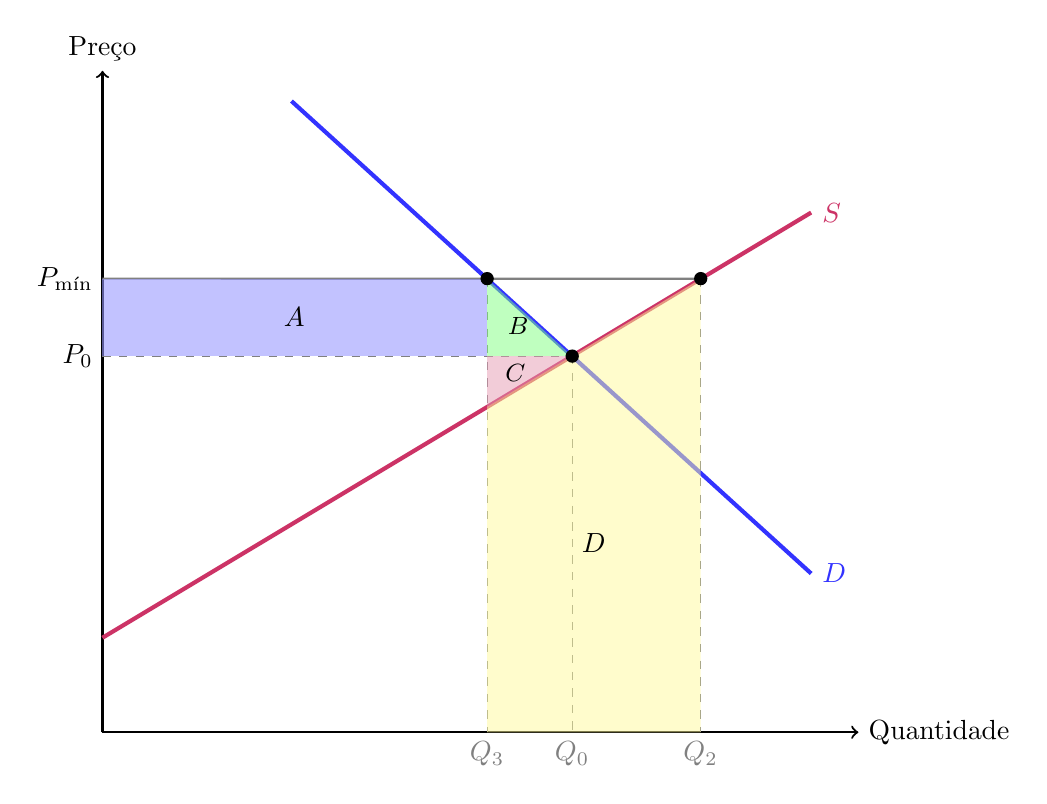
\begin{tikzpicture}[scale=1.2]
    % Eixos
    \draw[thick, ->] (0,0) -- (8,0) node[right] {Quantidade};
    \draw[thick, ->] (0,0) -- (0,7) node[above] {Preço};
    
    % Curva de Demanda (D) - movida para a direita, mais vertical
    % y = 8.5 - 0.909*x
    \draw[thick, blue!80, line width=1.5pt] (2.0,6.68) -- (7.5,1.68) node[right] {$D$};
    
    % Curva de Oferta (S) - inicia no eixo Y em (0, 1.0), mais vertical
    % y = 1.0 + 0.6*x
    \draw[thick, purple!80, line width=1.5pt] (0,1.0) -- (7.5,5.5) node[right] {$S$};
    
    % Interseção (equilíbrio de mercado) - calcular corretamente
    % 8.5 - 0.909*x = 1.0 + 0.6*x
    % 7.5 = 1.509*x
    % x = 4.97, y = 1.0 + 0.6*4.97 = 3.98
    \coordinate (E) at (4.97,3.98);
    
    % Preço de equilíbrio
    \coordinate (P0) at (0,3.98);
    \draw[dashed, gray] (P0) -- (E);
    \draw (0,3.98) node[left] {$P_0$};
    
    % Preço mínimo (acima do equilíbrio)
    \coordinate (Pmin) at (0,4.8);
    
    % Calcular Q3 e Q2 corretamente
    % Q3: interseção de Pmin=4.8 com demanda D: 4.8 = 8.5 - 0.909*x => x = 4.07
    % Q2: interseção de Pmin=4.8 com oferta S: 4.8 = 1.0 + 0.6*x => x = 6.33
    \coordinate (D3) at (4.07,4.8);
    \coordinate (S2) at (6.33,4.8);
    
    \draw[thick, gray] (Pmin) -- (6.33,4.8);
    \draw (0,4.8) node[left] {$P_{\text{mín}}$};
    
    % Quantidades
    \draw[dashed, gray] (4.07,4.8) -- (4.07,0) node[below] {$Q_3$};
    \draw[dashed, gray] (4.97,3.98) -- (4.97,0) node[below] {$Q_0$};
    \draw[dashed, gray] (6.33,4.8) -- (6.33,0) node[below] {$Q_2$};
    
    % Área A (retângulo - ganho dos produtores)
    \fill[blue!40, opacity=0.6] (0,3.98) rectangle (4.07,4.8);
    \node at (2.03,4.39) {$A$};
    
    % Triângulo B (perda de excedente do consumidor)
    \fill[green!50, opacity=0.5] (4.07,4.8) -- (4.97,3.98) -- (4.07,3.98) -- cycle;
    \node at (4.4,4.3) {\small $B$};
    
    % Triângulo C (perda de excedente do produtor - abaixo de P0 e acima da curva de oferta)
    % Pontos: (4.07, oferta em 4.07), (4.07, P0=3.98), (4.97, P0=3.98)
    % Oferta em x=4.07: y = 1.0 + 0.6*4.07 = 3.44
    % Centro: ((4.07+4.07+4.97)/3, (3.44+3.98+3.98)/3) = (4.37, 3.80)
    \fill[purple!40, opacity=0.5] (4.07,3.44) -- (4.07,3.98) -- (4.97,3.98) -- cycle;
    \node at (4.37,3.80) {\small $C$};
    
    % Área D (excesso de oferta/excedente não vendido)
    % Área entre Q3 e Q2, ABAIXO da curva de oferta S (entre a curva e o eixo X)
    % Oferta em x=4.07: y = 1.0 + 0.6*4.07 = 3.44
    % Oferta em x=6.33: y = 1.0 + 0.6*6.33 = 4.8
    % Desenha: começa em (Q3, 0), sobe pela curva de oferta até (Q2, oferta em Q2), desce até (Q2, 0)
    \fill[yellow!40, opacity=0.5] (4.07,0) -- plot[domain=4.07:6.33] (\x, {1.0 + 0.6*\x}) -- (6.33,0) -- cycle;
    \node at (5.2,2.0) {$D$};
    
    % Pontos principais
    \fill (E) circle (2pt);
    \fill (D3) circle (2pt);
    \fill (S2) circle (2pt);

\end{tikzpicture}

\end{document}
